
% TODO:
%    .append() with ignore_index=True
%     OR maybe just .reset_index(drop=True)   (more general purpose)
%
% memory diagrams, including .copy()

\chapter{Three kinds of aggregate data}

Now it's time to consider some loftier goals for our lowly atomic bits of data.
Most anything interesting in Data Science comes from arranging them together in
various ways to form more complex structures. This chapter is the subject of
these.

\index{aggregate data}
\section{Aggregate data types}

The number of ways in which pieces of data can be arranged is far greater than
the number of different atomic types. These various ways all have names, some
of them nerdy and/or exotic like ``hash tables,'' ``binary search trees,'' and
``skip lists.'' Nevertheless, there are again three basic ones which will form
the basis of our study: they're called \textbf{arrays}, \textbf{associative
arrays}, and \textbf{tables}. As before, we'll consider each one conceptually
first, and then look at how to use them in Python.

\index{array}
\subsection{Arrays}

An \textbf{array} is simply a sequence of items, all in a row. We call those
items the ``\textbf{elements}'' of the array. So an array could have ten whole
numbers as its elements, or a thousand strings of text, or a million real
numbers.

\index{homogeneous}
\index{heterogeneous}
Normally, we will deal with \textbf{homogeneous} arrays, in which all the
elements are of the same type; this turns out to be what you want 99\% of the
time. Some languages (including Python) do permit creating a
\textbf{heterogeneous} array, which could hold (say) three whole numbers,
sixteen reals, and four strings of text all mixed together. But usually you're
using an array to contain a bunch of related values, like the current balances
of all the accounts in your bank, or the Twitter screen names of all a user's
followees.

Figure~\ref{fig:array} shows what those two examples would look like
conceptually. One has four strings of text, and the other five real numbers.
Note that each \textit{entire set} of elements is \textit{one} variable. We
might call the left one ``\texttt{followees}'' and the right one
``\texttt{balances}.''

\begin{figure}[ht]
\centering
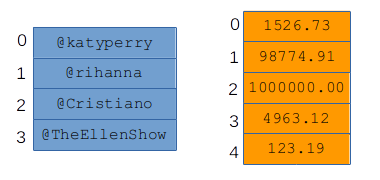
\includegraphics[width=0.6\textwidth]{array.png}
\caption{Two arrays.}
\label{fig:array}
\end{figure}

\index{index@index (pl:~indices)}
Worthy of special note are the numbers on the left-hand side. These numbers
are called the \textbf{indices} (singular:~\textbf{index}) of the array.
They exist simply so we have a way to talk about the individual elements. I
could say ``element \#2 of the \texttt{followees} array'' to refer to
\texttt{@Cristiano}.

\index{zero@zero, starting at}
And yes, you noticed that the index numbers start with 0, not 1. Yes, this is
weird. The reason I did that it is because nearly all programming languages
(including Python) number their array elements starting with zero, so you might
as well just start getting used to it now. It's really not hard once you get
past the initial weirdness.

Arrays are the most basic kind of aggregate data there is, and they are the
workhorse of a whole lot of Data Science processing. Sometimes they're called
\textbf{lists}, \textbf{vectors}, or \textbf{sequences}, by the way. (When a
particular concept has lots of different names, you know it's important.)

\index{array!associative}
\index{key-value pair}
\subsection{Associative arrays}

An \textbf{associative array}, by contrast, has no index numbers. And its
elements are slightly more complicated: instead of just bare values, an
associative array contains \textbf{key-value pairs}.
Figure~\ref{fig:assocArray} shows a couple of examples. The left-hand side of
each picture shows the keys, and the right-hand side the corresponding value.

With an associative array, you don't ask ``what's element \#3?'' like you do
with a regular array. Instead, you ask ``what value is associated with the
\texttt{"Washington"} key?'' And out pops your answer (\texttt{"Redskins"}).

\begin{figure}[ht]
\centering
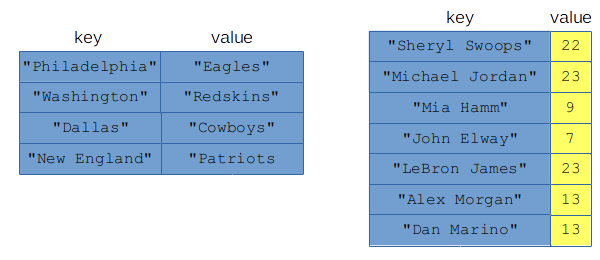
\includegraphics[width=0.9\textwidth]{assocArray.png}
\caption{Two associative arrays.}
\label{fig:assocArray}
\end{figure}

\index{order}
\index{undefined}
\index{mapping (a key to a value)}
All access to the associative array is through the keys: you can change the
value that goes with a key, retrieve the value that goes with a key, or even
retrieve and process \textit{all} the keys and their associated values
sequentially.\footnote{Using something called a ``loop,'' which we'll learn
about a little later in the book.} In that third case, the order in which
you'll receive the key-value pairs is \textbf{undefined} (which means ``not
guaranteed to be consistent'' or ``not necessarily what you'd expect.'') This
underscores the fact that there isn't any reliable ``first'' key-value pair,
or second, or last. They're just kind of all equally ``in there.'' Your mental
model of an associative array should just think of keys that are
\textbf{mapped} to values (we say that \texttt{"Dallas"} is ``mapped'' to
\texttt{"Cowboys"}) without any implied order. (Sure, the
\texttt{"Philadelphia"}/\texttt{"Eagles"} pair is at the top of the picture,
but that's only because I had to put \textit{something} at the top of the
picture, and I chose Philadelphia at random. It doesn't have any meaningful
primacy though.)

\index{homogeneous} Note a couple things about Figure~\ref{fig:assocArray}.
First, the keys in an associative array will almost always (and for us,
\textit{always}) be homogeneous. Similarly, the values will be homogeneous. But
the keys might not be of the same type as the values. In the left picture, both
keys and values are text, but in the right picture, the keys are text and the
values (uniform numbers of famous athletes) are whole numbers. This is
perfectly healthy and good.

\index{uniqueness!of keys in an associative array}
Second, realize that the \textit{keys} in an associative array must be
\textbf{unique} -- this means that there can be no duplicate keys. If we tried
to create a second \texttt{"Alex Morgan"} (oh, if only...) with a different
value, that new value would \textit{replace} Alex's current value, not sit
alongside the first one as an additional key-value pair.

The reverse is not true, however: the \textit{values} of an associative array
may very well not be unique. In the left-hand picture they are, but in the
right-hand picture there are duplicates: both Jordan and LeBron wore \#23 in
their stellar careers, while Hall of Famer quarterback Dan Marino once chose
the same uniform number that Alex wears today. This isn't a problem, because we
always access the information in an associative array \textit{through the
keys}. Asking ``what number did Mia Hamm wear?'' gives us a well-defined
answer. Asking ``which famous athlete wore \#23?'' does not. That's why we
can't ask that second question (and aren't meant to).

\subsection{Tables}

Lastly, we have the table, which in Data Science is positively ubiquitous. In
Figure~\ref{fig:table} we return to the pinterest.com example, with a table of
their most popular users. As you can see, it has more going on that than the
previous two aggregate data types. Still, it's pretty straightforward to wrap
your head around.

\begin{figure}[ht]
\centering
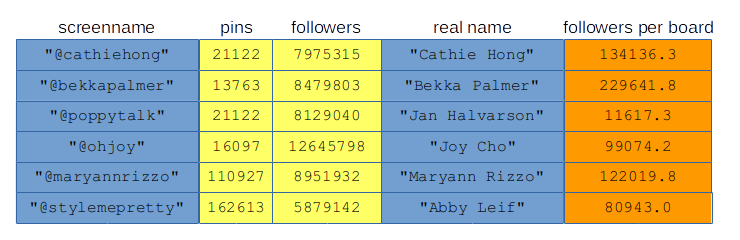
\includegraphics[width=\textwidth]{table.png}
\caption{A table.}
\label{fig:table}
\end{figure}

\index{row (of a table)}
\index{column (of a table)}
Unlike the other two aggregate data types, tables are full-on two-dimensional.
There's (theoretically) no limit to how many \textbf{rows} and how many
\textbf{columns} they can have. By the way, it's important to get those two
terms straight: rows go across, and columns go up and down. (Think of the
columns in the Trinkle Rotunda.) Also, the typical table has many, many more
rows than columns, so they're super tall and skinny, not short and fat.

\index{heterogeneous}
\index{homogeneous}
Although the \textit{rows} of a table are often heterogeneous, each
\textit{column} must be homogeneous. You can see that with a glance at
Figure~\ref{fig:table}. Each column represents a specific type of data -- in
this case, some statistic or piece of information about a Pinterest user.
Clearly all screen names should be of a text type, all ``number of pins or
followers'' should be whole numbers, \textit{etc.} It doesn't make sense
otherwise.

\index{order}
As with the other types, the whole dog-gone table -- no matter how many
millions of rows it might have -- is \textit{one} variable with a single name.
Also, just like with associative arrays, there normally isn't any implied
\textit{order} to the rows. Many implementations of these data types (including
Pandas) will actually let you specify ``the first row'' or ``the
$53^{\textrm{rd}}$ row,'' but that always makes me cringe because conceptually,
there isn't any such thing. They're all just ``rows'' that are all ``in
there.''

\subsubsection{``Querying'' tables (and other things)}
\index{query}
Now you might be wondering how to actually ``get at'' the individual values of
a table. Unlike arrays, there's no index number. And unlike associative arrays,
there's no key. How then to address, say, the \texttt{@poppytalk} row?

The answer will turn out to be something called a \textbf{query}, which is a
geeky way of saying ``a set of criteria which will match some, but not all, of
the rows and/or columns.'' For instance, we might say ``tell me the pin count
for \texttt{@ohjoy}.'' Or, ``give me all the information for any user who has
more than 100,000 followers per board \textit{and} at least 20,000 pins.''
Those specific requirements will restrict the table to a subset of its rows
and/or columns. We'll learn the syntax for that later. It's a bit tricky but
very powerful.

\section{Aggregate data and memory pictures}

\subsection{Associative arrays}

\subsection{Data frames}

\section{The three kinds in Python}

\subsection{Arrays: \texttt{numpy}'s \texttt{ndarray}}

% np.array([]), np.arange(), np.zeros(),
% np.loadtxt("file", dtype=object, delimiter='!!!')

% indexing, slices

\subsection{Associative arrays: Python's \texttt{dict}}

\subsection{Data frames: \texttt{pandas}'s \texttt{DataFrame}}


% Somewhere: .map() for recoding

